\documentclass[tikz,border=2pt]{standalone}
\usepackage{amsmath,amssymb}
\usepackage{tikz}

\begin{document}
% Connected: every pair of vertices is joined by some path. Unconnected: the vertices split
% into pieces with no edge between them.
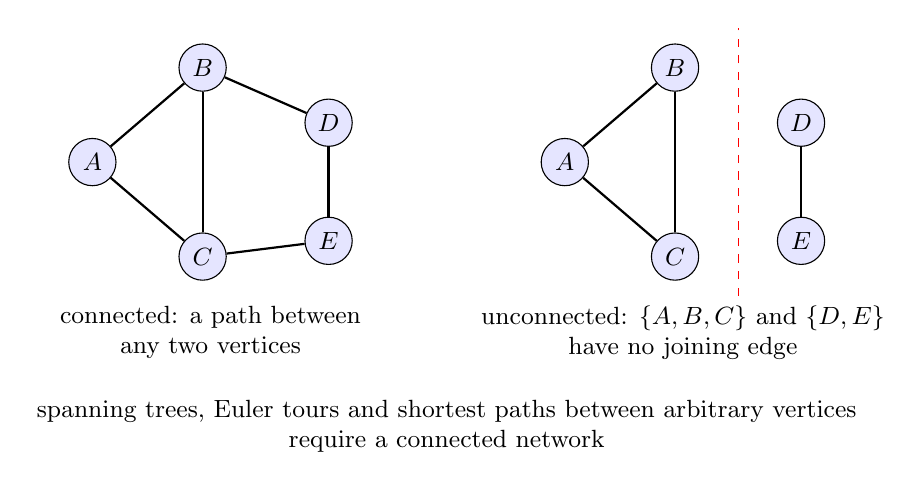
\begin{tikzpicture}[every node/.style={font=\small}, v/.style={draw, circle, fill=blue!10, minimum size=6mm, inner sep=0pt}]
	\begin{scope}
		\node[v] (A) at (0,0) {$A$}; \node[v] (B) at (1.4,1.2) {$B$}; \node[v] (C) at (1.4,-1.2) {$C$}; \node[v] (D) at (3,0.5) {$D$}; \node[v] (E) at (3,-1.0) {$E$};
		\foreach \a/\b in {A/B, A/C, B/D, C/E, D/E, B/C} {\draw[thick] (\a) -- (\b);}
		\node[anchor=north, align=center] at (1.5,-1.7) {connected: a path between\\ any two vertices};
	\end{scope}
	\begin{scope}[xshift=6cm]
		\node[v] (A) at (0,0) {$A$}; \node[v] (B) at (1.4,1.2) {$B$}; \node[v] (C) at (1.4,-1.2) {$C$}; \node[v] (D) at (3,0.5) {$D$}; \node[v] (E) at (3,-1.0) {$E$};
		\foreach \a/\b in {A/B, A/C, B/C, D/E} {\draw[thick] (\a) -- (\b);}
		\draw[red, dashed] (2.2,-1.7) -- (2.2,1.7);
		\node[anchor=north, align=center] at (1.5,-1.7) {unconnected: $\{A,B,C\}$ and $\{D,E\}$\\ have no joining edge};
	\end{scope}
	\node[anchor=north, align=center] at (4.5,-2.9) {spanning trees, Euler tours and shortest paths between arbitrary vertices\\ require a connected network};
\end{tikzpicture}
\end{document}
